\documentclass[14pt]{article}
\usepackage{../../report-tex/styles}


\begin{document}

\titlewithlabnum{1}

\tableofcontents
\newpage

\section{Мета:}
Отримати навички створення програм для Windows на основі проектів API
Win32 для Visual C++ і навчитися модульному програмуванню на C++.
\section{Завдання:}
\begin{enumerate}
    \item Створити у середовищі MS Visual Studio C++ проект Win32 з ім’ям Lab1.
    \item Написати вихідний текст програми згідно варіантів завдання.
    \item Скомпілювати вихідний текст і отримати виконуваний файл програми.
    \item Перевірити роботу програми
\end{enumerate}

\begin{align}
    B_1 &= 22 \bmod 4 = 2 \\
    B_2 &= (22+1) \bmod 4 = 3    
\end{align}

\subsection{Варіант 2:}
Два вікна діалогу. Спочатку
з’являється перше, яке має дві
кнопки: [Далі >] і [Відміна].
Якщо натиснути кнопку [Далі
>], то воно закриється і
з’явиться друге длг вікно, яке
має кнопки: [< Назад], [Так] і
[Відміна]. Якщо натиснути
кнопку [<Назад], вікно
закриється і перехід до
першого вікна.
\subsection{Варіант 3:}
Вікно діалогу з елементом
списку (List Box) та двома
кнопками: [Так] і [Відміна]. У
список автоматично
записуються назви груп
нашого факультету. Якщо
вибрати потрібний рядок
списку і натиснути [Так], то у
головному вікні повинен
відображатися текст
вибраного рядка списку.

\section{Текст програми:}
\subsection{Module: com.github.erotourtes.drawing.editor}
\lstinputlistingukr{DmProcessor.kt}{../src/main/kotlin/com/github/erotourtes/drawing/editor/DmProcessor.kt}
\lstinputlistingukr{Editor.kt}{../src/main/kotlin/com/github/erotourtes/drawing/editor/Editor.kt}
\lstinputlistingukr{Editors.kt}{../src/main/kotlin/com/github/erotourtes/drawing/editor/Editors.kt}
\lstinputlistingukr{ShapesList.kt}{../src/main/kotlin/com/github/erotourtes/drawing/editor/ShapesList.kt}

\subsection{Module: 1.0}
\lstinputlistingukr{MANIFEST.MF}{../src/main/resources/META-INF/MANIFEST.MF}

\subsection{Module: com.github.erotourtes.view}
\lstinputlistingukr{MainController.kt}{../src/main/kotlin/com/github/erotourtes/view/MainController.kt}
\lstinputlistingukr{MainView.kt}{../src/main/kotlin/com/github/erotourtes/view/MainView.kt}
\lstinputlistingukr{MenuBar.kt}{../src/main/kotlin/com/github/erotourtes/view/MenuBar.kt}
\lstinputlistingukr{ToolBar.kt}{../src/main/kotlin/com/github/erotourtes/view/ToolBar.kt}

\subsection{Module: com.github.erotourtes.app}
\lstinputlistingukr{MyApp.kt}{../src/main/kotlin/com/github/erotourtes/app/MyApp.kt}

\subsection{Module: com.github.erotourtes.drawing}
\lstinputlistingukr{CanvasPane.kt}{../src/main/kotlin/com/github/erotourtes/drawing/CanvasPane.kt}
\lstinputlistingukr{EditorHandler.kt}{../src/main/kotlin/com/github/erotourtes/drawing/EditorHandler.kt}

\subsection{Module: com.github.erotourtes.drawing.shape}
\lstinputlistingukr{Shape.kt}{../src/main/kotlin/com/github/erotourtes/drawing/shape/Shape.kt}
\lstinputlistingukr{Shapes.kt}{../src/main/kotlin/com/github/erotourtes/drawing/shape/Shapes.kt}

\subsection{Module: com.github.erotourtes.styles}
\lstinputlistingukr{ToolbarStyles.kt}{../src/main/kotlin/com/github/erotourtes/styles/ToolbarStyles.kt}

\subsection{Module: com.github.erotourtes.utils}
\lstinputlistingukr{Dimension.kt}{../src/main/kotlin/com/github/erotourtes/utils/Dimension.kt}
\lstinputlistingukr{ExtensionFunctions.kt}{../src/main/kotlin/com/github/erotourtes/utils/ExtensionFunctions.kt}
\lstinputlistingukr{Utils.kt}{../src/main/kotlin/com/github/erotourtes/utils/Utils.kt}



\section{Ілюстрації:}
\begin{figure}[H]
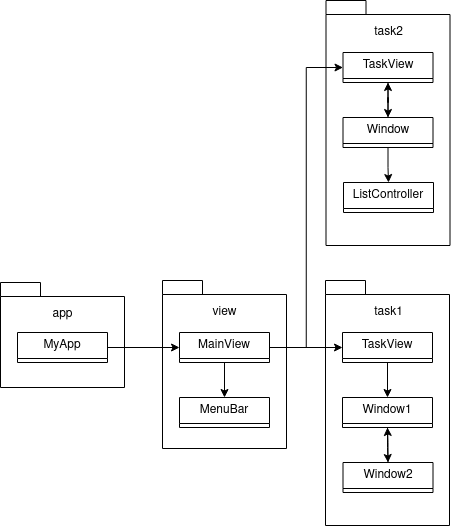
\includegraphics[width=10cm]{1}
\centering
\end{figure}


\section{Висновки:}
Отже, я отримав навички створення програм для Linux і навчився модульному програмуванню на Kotlin.

\end{document}
